\section{Introduction}


\subsection{Description of the Task}
In this report the segmentation of wooden planks with images of 256x3072 pixels are investigated for a real-time analysis task. The motivation for this report is the creation of a complete hardware and software system for a real-time damage detection on coated wooden planks in a fully automatized factory for built-in kitchen furniture.\\
The task is to detect damages due to a coating process on wooden planks. In order to be able to adjust the sensitivity of the detection, it is divided into two main tasks. The first task is the segmentation of the image in order to find the wooden plank inside the image. The second task is the actual detecting of the damage. This should be easily accomplished by a simple threshold. Therefore, this work will focus on the more complicated part, creating and training a Convolutional Neural Network (CNN) for the purpose of the segmentation. For the training, real example pictures (\ref{pic:ExampleImage}) of automatically coated wooden planks were used. The Segmentation Network should find these planks in a picture section and distinguish them from the conveyor belt system in the background.
\begin{center}\begin{minipage}[t]{\textwidth}
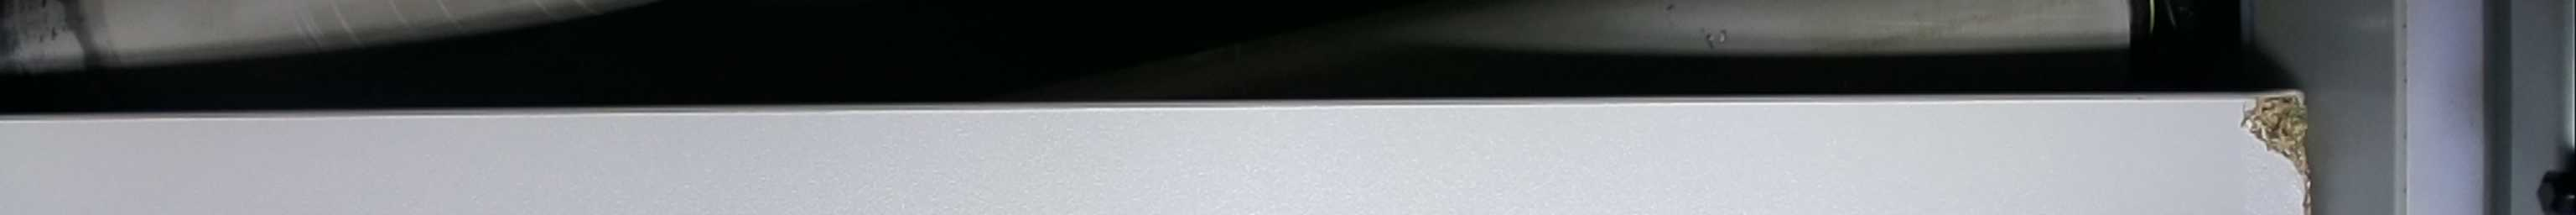
\includegraphics[width=\textwidth]{Images/ExampleImage.png}\label{pic:ExampleImage}

\includegraphics[width=\textwidth]{Images/m_ExampleLabel1.png}\label{pic:ExampleLabel1}
\captionof{figure}{Example of a white coated wooden plank with an error on the top right corner together with its corresponding mask}
\vspace{0.5cm}
\end{minipage}\end{center}
\begin{center}\begin{minipage}[t]{\textwidth}
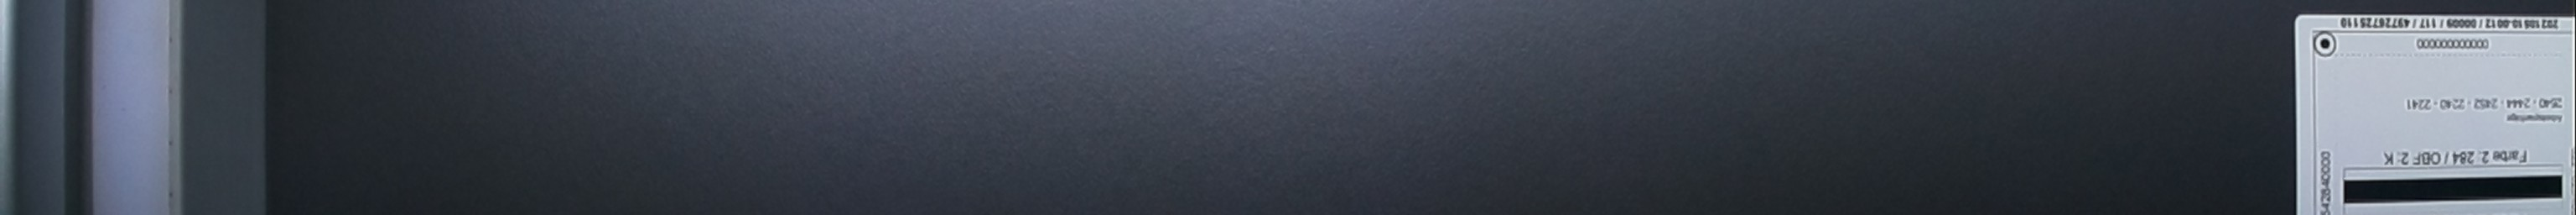
\includegraphics[width=\textwidth]{Images/ExampleImage2.png}\label{pic:ExampleImage2}

\includegraphics[width=\textwidth]{Images/m_ExampleLabel2.png}\label{pic:ExampleLabel2}
\captionof{figure}{Example of a black coated wooden plank with a bar-code label together with its corresponding mask}
\end{minipage}\end{center}
\subsection{Approach to the Solution}
For the approach to the solution of this problem, at first, a pre-trained encoder with a small decoder as segmentaion network was applied. Therefore, several pre-trained encoders of the \verb|Tensorflow| library were investigated and later on different decoder structures tested. Additional to this simple Fast-forward CNNs \cite{JonathanLong.} smaller, self-edited codes for more complex Segmentation Network Architectures were researched, like the U-Net\cite{Ronneberger.2015} and the SegNet\cite{Badrinarayanan.2017}.\\
The original example set contains 126 pictures of the size 256x3072, which is further referred to as 'big images'. In a data generation process, the images were flipped and shifted, in order to generate more data for the training. Because of the usage of pre-trained encoders, which have a build-in input (no further layers were included on the input-side of the encoders), the original image (\ref{pic:ExampleImage}) with a size of 256x3072 pixels is split into 12 images of 256x256 pixels, further referred to as 'sliced images'.\\
Since some of the planks have bar code labels, two setups are considered. At first we only aim to distinguish planks from the background (single-class setup). In order to get rid of the confusion around labels we separate planks, labels, and background (multi-class setup).\\
In all test setups, unless stated otherwise, \verb|BinaryCrossentropy| is used as loss function for single-classification while \verb|SparseCategoricalCrossentropy| is applied for the multi-classification. The used optimizer for the compiling of the models is the \verb|adam| optimizer, based on stochastic gradient descent scheme. The learning rate is not set for in any of these investigations, so it is always set to 0.001 as a standard setting in \verb|Keras| (\url{https://keras.io/api/optimizers/adam/}). As activation function \verb|SELU| was applied in nearly all of the layers, except when different activations should be tested (as \verb|ReLU| in \cref{subsec:SegNet}).\\
The amount of total parameters and trainable parameters for each model trained in this project can be found in the appendix (\cref{tab:ParameterSummary}).